\documentclass{beamer}
 
\usepackage[american]{babel}
\usepackage[utf8]{inputenc}
\usepackage[T1]{fontenc}
\usetheme{Copenhagen}
\setbeamertemplate{navigation symbols}{}
%\title[Translittération automatique]{Données Séquentielles et Symboliques: Translittération automatique}
\title[Machine Transliteration]{Sequential Symbolic Data: Machine Transliteration}
\author[A.~Bérard, M.~Millet, C.~Robin]{Alexandre Bérard, Mathias Millet, Charles Robin}

\date{January 10th, 2014}

\newcommand*\oldmacro{}%
\let\oldmacro\insertshorttitle%
\renewcommand*\insertshorttitle{%
  \oldmacro\hfill%
  \insertframenumber\,/\,\inserttotalframenumber}

\begin{document}

\begin{frame}
\titlepage
\end{frame}

\section{Introduction}   
 
\begin{frame}
    \frametitle{Introduction}
	\framesubtitle{Translitération}
	\begin{block}{Definition}
	    \begin{itemize}
    		\item Conserver la m\^eme prononciation pour un mot
    		\item En utilisant des phonèmes d'une autre langue
    		\end{itemize}
    \end{block}	    
    
	\begin{exampleblock}{Examples : anglais - hindi}
	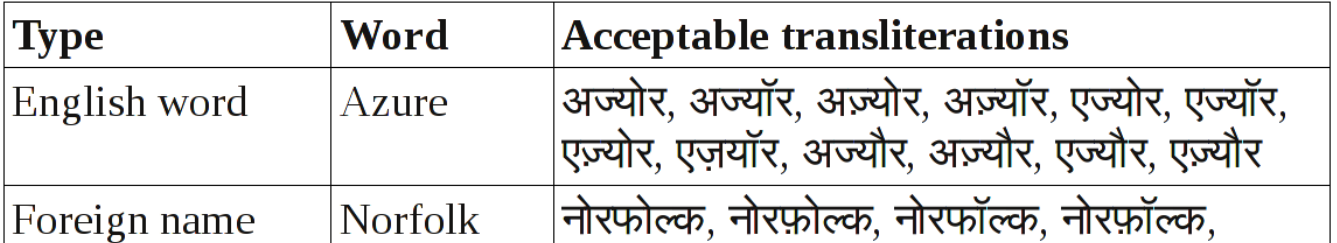
\includegraphics[scale=0.3]{en-in-example}
    \end{exampleblock}
    
	\begin{block}{Pourquoi ?}
	\begin{itemize}
		\item Traduction automatique de termes techniques
		\item Plus besoin de maintenir un dictionnaire !
	\end{itemize}
	\end{block}	    
    
    
\end{frame}

\begin{frame}
\frametitle{Introduction}
\framesubtitle{Le projet}

	\begin{block}{Le but}
		Implémenter des techniques de translitération 
		\begin{itemize}
		\item Entre l'espagnol et le portugais
		\item Entre l'anglais et le russe
		\end{itemize}
	\end{block}

	\begin{block}{Les données}
	Pour chaque pair de languages :		
		\begin{itemize}
		\item Un corpus d'apprentissage
		\item Un corpus de test
		\end{itemize}		
	\end{block}

\end{frame}

\section{Méthodologie}

\begin{frame}
\frametitle{Méthodologie}

	\begin{block}{Échantillonage ?}
	Les données fournies sont déjà séparées entre données d'apprentissage et données de test\\
	$\Longrightarrow$ L'échantillonage n'est pas nécéssaire
	\end{block}

	\begin{block}{Mesures}
		
	
	\end{block}


\end{frame}



\begin{frame}
    \frametitle{Bibliography}
    {\fontsize{0.8em}{1em}
    \nocite{*}
    \bibliographystyle{plain}
    \bibliography{report}}
\end{frame}

\begin{frame}
    \frametitle{Overview}
\end{frame}

\section{Conclusion}
\begin{frame}
    \frametitle{Conclusion}
    \url{https://code.google.com/p/transliteration}
\end{frame}

\end{document}
